\chapter{Kalibrace}

\section{Autokalibrace úrovní}
Vzhledem k omezenému množství paměti RAM v použitém mikrokontroléru a omezenému výkonu se při použití bez počítače používá pouze autokalibrace napěťových úrovní. Ty se detekují během autokalibračního kroku se standardem open. Touto metodou jsou získány napěťové úrovně odpovídající koeficientům odrazu $\Gamma=\SI{1}{}$ a $\Gamma=\SI{-1}{}$. Takto získané úrovně jsou použity pro zobrazení měřených dat do rozsahu $\Gamma\in\left\langle 1, -1 \right\rangle $ pomocí bilineárního mapování podle rovnice \ref{equation_normalization}.Tímto krokem je téměř odstraněn případný stejnosměrný posuv změřených dat, zároveň jsou data znormována. Tato autokalibrace však probíhá pouze pro dvě statické hodnoty, jedná se tedy prakticky o stejnosměrné měření a ne vždy přesně odpovídá pozdějším měřením, které již probíhají při zapnutém budicím signálu. Po této autokalibraci tedy stále může být v zobrazovaných datech přítomna stejnosměrná složka, případně nemusí plně odpovídat koeficient odrazu. Podle opakovaných testů s kalibračními standardy \quotedblbase short\textquotedblleft{} a \quotedblbase open\textquotedblleft{} je však tato chyba normování typicky menší než $\Delta\Gamma=\pm\SI{0.1}{}$. Tato autokalibrace probíhá ve firmware, používá ji i software, dokud není provedena OSL kalibrace. Změřené průběhy pro všechny tři kalibrační standardy po autokalibraci jsou zaneseny v grafu \ref{standards_after_autocalibration}. Na všech třech průbězích je vidět shodné zvlnění, stejnosměrný posuv a chyba normalizace.

\begin{equation}
\begin{gathered}
	\Gamma[n]=2\cdot\dfrac{U[n]-U_\mathrm{short}}{U_\mathrm{open}-U_\mathrm{short}} -1
\end{gathered}
\label{equation_normalization}
\end{equation}

\begin{figure}[htbp]
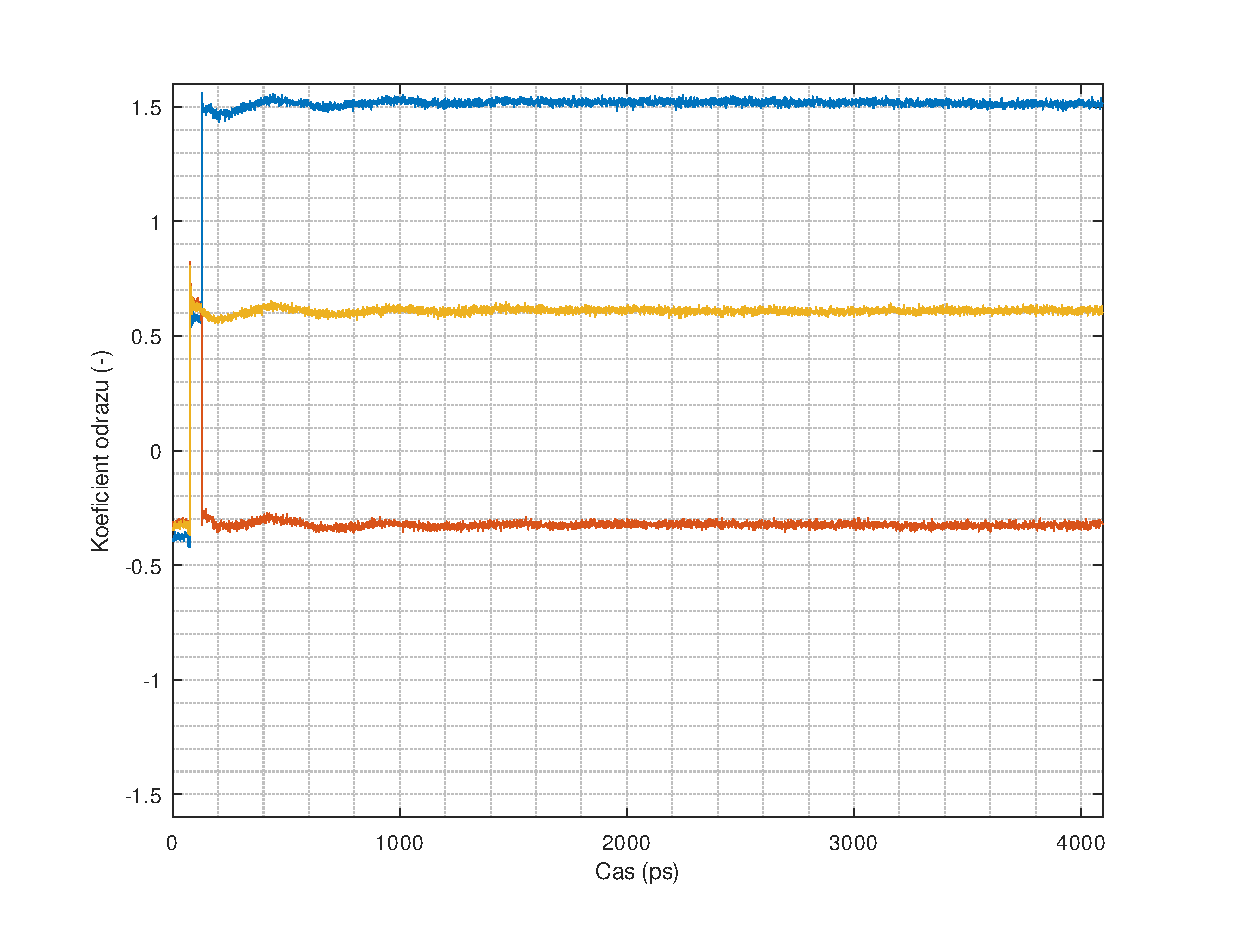
\includegraphics[width=\textwidth,keepaspectratio]{images/gui/standards_after_autocalibration.eps}\caption{Průběhy odpovídající změřeným standardům po autokalibraci. Modře je označen průběh odpovídající kalibru \quotedblbase open\textquotedblleft , červeně pro kalibr \quotedblbase short\textquotedblleft{} a žlutě pro kalibr \quotedblbase load\textquotedblleft .}\label{standards_after_autocalibration}
\end{figure}

\begin{figure}[htbp]
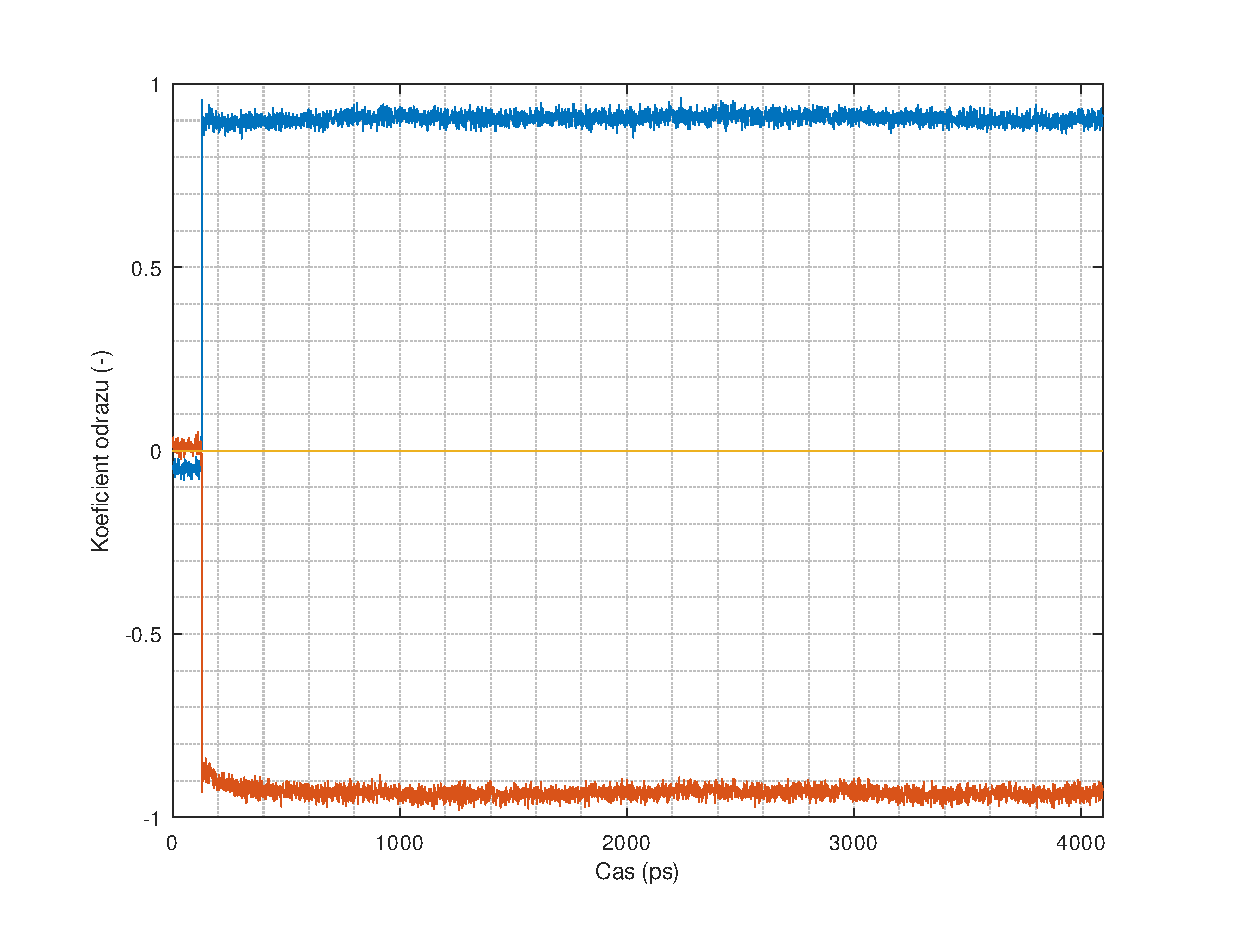
\includegraphics[width=\textwidth,keepaspectratio]{images/gui/standards_after_load_calibration.eps}\caption{Průběhy odpovídající změřeným standardům po základní kalibraci. Modře je označen průběh odpovídající kalibru \quotedblbase open\textquotedblleft , červeně pro kalibr \quotedblbase short\textquotedblleft{} a žlutě pro kalibr \quotedblbase load\textquotedblleft .}\label{standards_after_load_calibration}
\end{figure}

\section{Základní kalibrace pomocí standardu \quotedblbase open\textquotedblleft}
Jako základní metoda kalibrace pro potlačení zvlnění a stejnosměrného posuvu byla zvolena kalibrace pomocí standardu \quotedblbase load\textquotedblleft . V grafu \ref{standards_after_load_calibration} jsou vidět průběhy po základní kalibraci provedené pomocí odečtení změřeného průběhu pro kalibr \quotedblbase load\textquotedblleft{} od všech třech průběhů. Ve změřených datech tak bylo výrazně potlačeno zvlnění a stejnosměrný posuv. Zároveň byl z měřených dat odstraněn budicí pulz. Tato základní metoda kalibrace je automaticky aplikována, jakmile uživatel provede kalibraci se standardem \quotedblbase load\textquotedblleft{} a uloží kalibrační data pro tento standard. Jak je však vidět v grafu, nedochází k opravě chybné normalizace.

\section{Kalibrace typu OSL}

\subsection{Chybový model}
Systematické chyby měření reflektometru jsou idealizovány pomocí lineárního dvoubranu, který je virtuálně vložen mezi idealizovaný měřicí port reflektometru a \acrshort{DUT}. Tento model a odvození odstranění jeho vlivu byl převzat z \cite{time_domain_analyzer_calibration} a \cite{time_domain_analyzer_calibration_normalization}. Znázornění chybového modelu se nachází v grafu \ref{error_model}. Jako $a_0$ je označena napěťová vlna z generátoru budicích pulzů, $b_0$ je napěťová vlna měřená reflektometrem. Chybový model jeuvažován pro práci ve frekvenční doméně. S-parametr měřený reflektometrem je označen jako $S_\mathrm{M}$. Skutečný S-parametr DUT je uveden jako $S_\mathrm{A}$. Chybový model obsahuje čtyři chybové parametry, přičemž jeden byl normalizován na 1 a stal se součástí jednoho ze třech zbývajících parametrů, a sice $E_\textrm{R}$. Pro jednostranné měření, které se používá pro reflektometr pracující pouze v režimu TDR a nikoli \acrshort{TDT}, je možné takto redukovat počet stupňů volnosti a ke kalibraci tak stačí pouze tři mechanické kalibry místo čtyř. Parametr $E_\textrm{D}$ je chyba direktivity, která vyjadřuje prosakování budicího pulzu do měřených dat. Parametr $E_\textrm{R}$ je sdružená chyba dopředného a zpětného přenosu chybového dvoubranu, vyjadřuje útlum mezi reflektometrem a DUT, který je způsobený např. útlumem použitého vedení. Parametr $E_\textrm{S}$ vyjadřuje odraz od reflektometru, popř. jeho prodlužovacího vedení.
\begin{figure}[htbp]
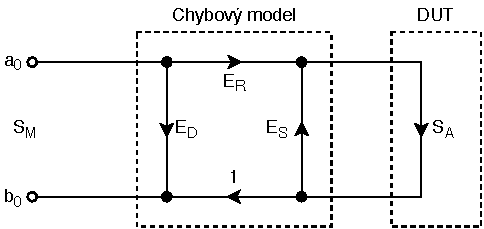
\includegraphics[width=0.7\textwidth,keepaspectratio]{images/error_box.pdf}\caption{Chybový model reflektometru.}\label{error_model}
\end{figure}

Podle \cite{time_domain_analyzer_calibration_normalization} odpovídá měřený koeficient odrazu
\begin{equation}
\begin{gathered}
	S_\mathrm{M} = E_\textrm{D} + E_\textrm{R} \left( \dfrac{S_\mathrm{A}}{1-E_\mathrm{S} S_\mathrm{A}} \right). 
\end{gathered}
\end{equation}

Z této rovnice je možné získat skutečný koeficient odrazu měřeného DUT
\begin{equation}
\begin{gathered}
	S_\mathrm{A} = \dfrac{S_\mathrm{M} - E_\textrm{D}}{E_\textrm{R} + E_\textrm{S} \left( S_\mathrm{M} - E_\textrm{D} \right) }.
\end{gathered}
\label{equation_s_parameter_calibration}
\end{equation}

Pro idealizované mechanické kalibry je možné jednoduše získat parametry chybového modelu pomocí dosazení jejich idealizovaných S-parametrů
\begin{equation}
\begin{gathered}
S_\mathrm{M}=
   \begin{dcases}
	S_\mathrm{ML} = E_\textrm{D} & S_\mathrm{A}=0	\\
	S_\mathrm{MO} = E_\textrm{D} + \dfrac{E_\textrm{R}}{1-E_\mathrm{S}}  & S_\mathrm{A}=+1	\\
	S_\mathrm{MS} = E_\textrm{D} - \dfrac{E_\textrm{R}}{1+E_\mathrm{S}}  & S_\mathrm{A}=-1.
   \end{dcases}
\end{gathered}
\end{equation}

Pak je možné odvodit výpočty jednotlivých chybových parametrů
\begin{equation}
\begin{gathered}
   E_\textrm{D}=S_\mathrm{ML} \\
   E_\mathrm{S}=\dfrac{\left( \dfrac{S_\mathrm{MO}-S_\mathrm{ML}}{S_\mathrm{MS}-S_\mathrm{ML}}\right)  +1}{\left( \dfrac{S_\mathrm{MO}-S_\mathrm{ML}}{S_\mathrm{MS}-S_\mathrm{ML}}\right) -1} = \dfrac{S_\mathrm{MO} + S_\mathrm{MS} -2\cdot S_\mathrm{ML}}{S_\mathrm{MO} - S_\mathrm{MS}} \\
   E_\mathrm{R}=\dfrac{2}{\left( \dfrac{1}{S_\mathrm{MO}-S_\mathrm{ML}}\right)  - \left( \dfrac{1}{S_\mathrm{MS}-S_\mathrm{ML}} \right) } = \dfrac{\left( S_\mathrm{MS} - S_\mathrm{ML} \right) \cdot \left( S_\mathrm{MO} - S_\mathrm{ML} \right) }{S_\mathrm{MS} - S_\mathrm{MO}}.
\end{gathered}
\end{equation}

Pro kalibraci je tedy nezbytné změřit tři kalibrační standardy, výsledkem jsou tři sady S-parametrů, jejichž dosazením do vzorce \ref{equation_s_parameter_calibration} získáme skutečné S-parametry měřeného DUT. Kalibrace probíhá ve frekvenční doméně, pro kalibraci je tedy nezbytné změřená data jednotlivých kalibrů i DUT převést pomocí Fourierovy transformace do frekvenční domény, provést kalibraci a převést inverzní Fourierovou transformací zpět do časové domény.

Pokud se za měřená data dosadí jeden z použitých kalibrů, je výsledkem odpovídající koeficient odrazu v $t=0$, což bylo ověřeno i symbolicky pomocí matematického symbolického nástroje wxMaxima. Bohužel pro jiná měřená data již výsledek neodpovídá očekávání, nepovedlo se zjistit, proč tomu tak je. Software tak má tedy implementovanou kalibrační metodu OSL, avšak z neznámých důvodů nepracuje dle očekávání.
